\documentclass{article}
\usepackage{preamble}
\input{preamble}
\graphicspath{ {images/} }
%%%%%%%%%%%%%%%% Document %%%%%%%%%%%%%%%%
\begin{document}
\begin{center}
{\huge \underline{Data Analysis}}
\end{center}

\section*{Linear Algebra Refresher}
\begin{theorem}[Rank Theorem] \hphantom{}
  \begin{itemize}
  \item Let $A \in \mathbb{R}^{m \times  n}, B  \in \mathbb{R}^{n \times  k}$, with $\myrank(B) = n$. Then $\myrank(AB) = \myrank(A)$. 
  \item Let $A \in \mathbb{R}^{m \times  n}, C \in \mathbb{R}^{\ell \times  m}$, with $\myrank(C) = n$. Then $\myrank(CA) = \myrank(A)$.  
\end{itemize}
\end{theorem}

\subsection{Lagrange Multipliers - Mine}
\begin{theorem}[Single Constraint Lagrange Multiplier]
Let $f: \mathbb{R}^{n} \to \mathbb{R}$ be a function we wish to minimize under the constraint $g =0$, with $g: \mathbb{R}^{n} \to \mathbb{R}$.  
\begin{figure}[H] \centering 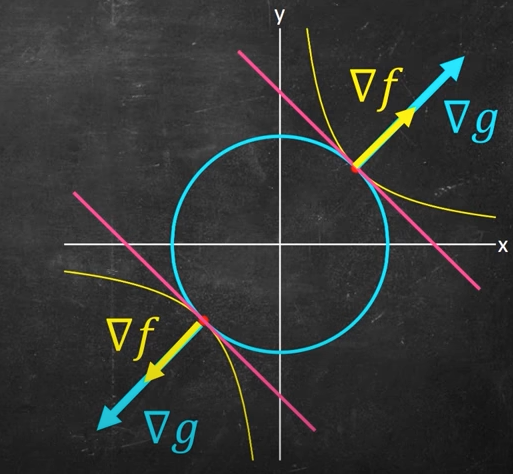
\includegraphics[height=0.2\textheight,width=0.9\textwidth,keepaspectratio]{lagrangianSingleConstraint} \caption{Lagrangian single constraint} \label{fig:lagrangianSingleConstraint} \end{figure}
At a critical point, we would have:
\[
  \bm{\nabla}f = \lambda \bm{\nabla}g
\]
for some $\lambda \in \mathbb{R}$. 

Equivalently, we can define the Lagrangian:
\[
  \mathcal{L}(x,\lambda) = f(x) + \lambda g(x)
\]
and then look for stationary points, i.e. points that satisfy:
\[
  \frac{\partial \mathcal{L}}{\partial x} = 0 \quad and \quad \frac{\partial \mathcal{L}}{\partial \lambda} = 0  
\]

\end{theorem}
\begin{theorem}[Multiple Constraints Lagrange Multipliers]
Now assume we wish to minimize $f: \mathbb{R}^{3} \to \mathbb{R}$, under constraints of both $g_1 = 0$ and $g_2 = 0$, with $g_1, g_2: \mathbb{R}^{3} \to \mathbb{R}$. 

\begin{figure}[H] \centering 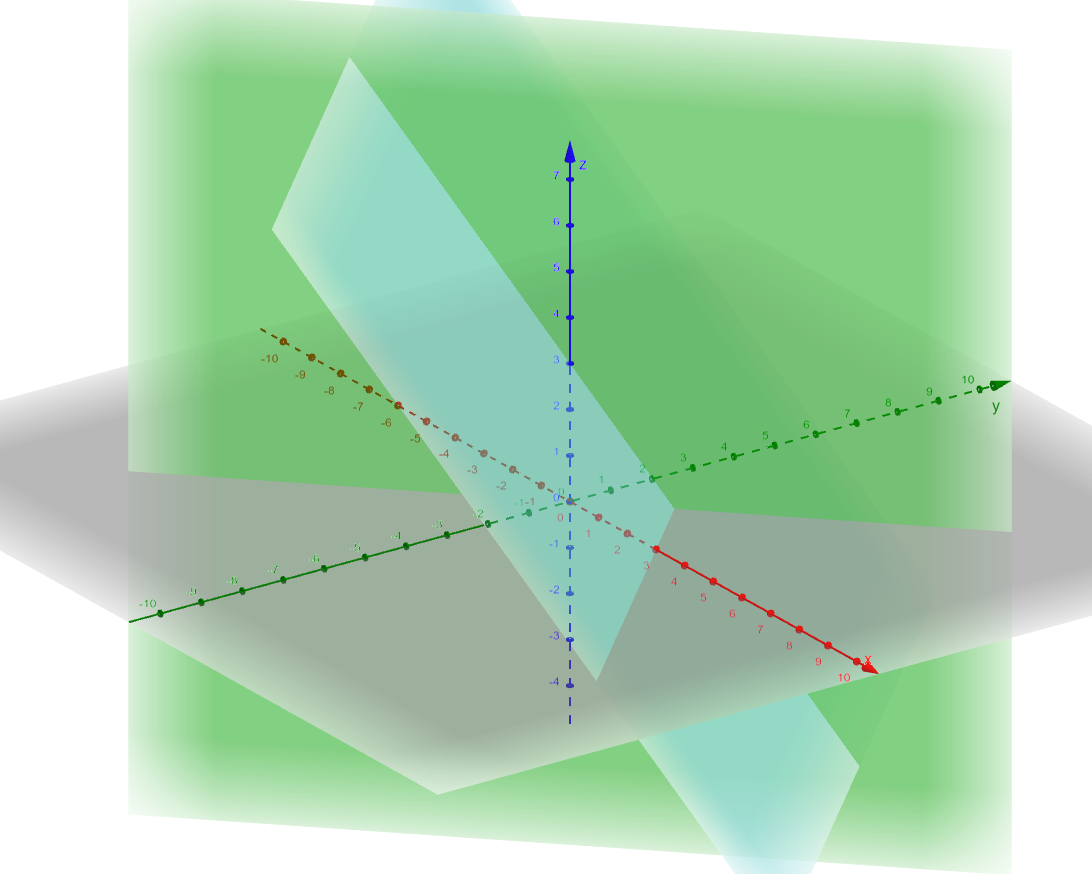
\includegraphics[height=0.2\textheight,width=0.9\textwidth,keepaspectratio]{lagrangeMultipleConstraints} \caption{The constraints $g_1 =0$ and $g_2=0$ visualized. \\ \href{https://www.geogebra.org/3d/nxbqmx2g}{https://www.geogebra.org/3d/nxbqmx2g}} \label{fig:lagrangeMultipleConstraints} \end{figure}
Every point $\bm{x}$ on the constraint-surface of a constraint $g_i$ has a space of allowable directions we can walk along. 
Note that this space is given by all vectors perpendicular to $\bm{\nabla}g_i (\bm{x})$. 
Therefore, the set of directions that are allowed by \textit{all} constraints is the space of directions that are perpendicular to \textit{all} the gradients. 
Let's denote the span of the gradients by $S$, and the set of allowable directions by $A$.
Then $A = S^{\perp}$.
\begin{figure}[H] \centering 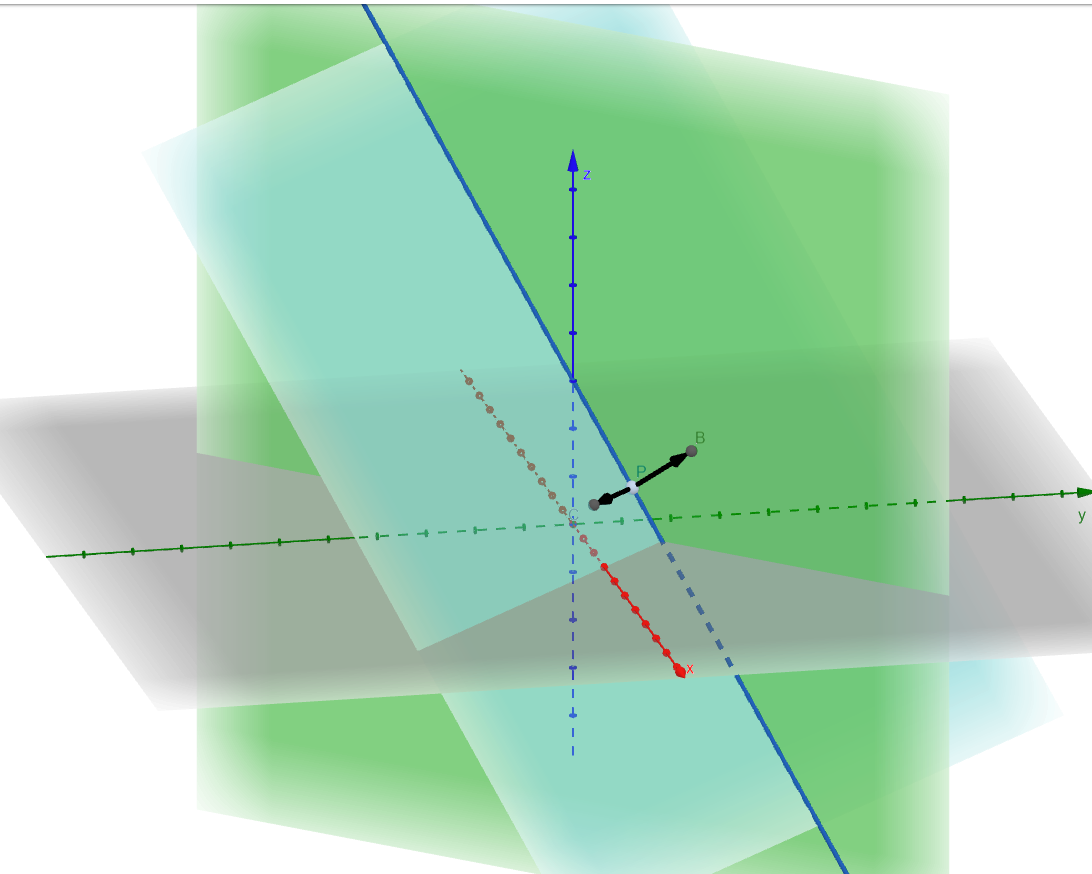
\includegraphics[height=0.3\textheight,width=0.9\textwidth,keepaspectratio]{lagrangeMultipleAllowable2} \caption{The blue line $A$ represents all allowable directions. The plane perpendicular to it (not shown) is $S$. } \label{fig:lagrangeMultipleAllowable2} \end{figure}
We are interested in points where $f$ does not change as we walk. I.e. in the set of our allowed directions $A$, $f$ does not change.
Specifically, this means that $\bm{\nabla}f \in A^{\perp} = S$. Thus, there are scalars $\lambda_1, \lambda_2$ such that:
\[
  \bm{\nabla}f(\bm{x}) = \sum_{i=1}^{2} \lambda_i \bm{\nabla}g_i(\bm{x})
\]

More generally, for $f: \mathbb{R}^{n} \to \mathbb{R}$ with $m$ constraints $g_i: \mathbb{R}^{n} \to \mathbb{R}$ we look for $\lambda_1, \ldots  \lambda_m$ s.t.:
\[
  \bm{\nabla}f(\bm{x}) = \sum_{k=1}^{m} \lambda_k \bm{\nabla}g_{k} (\bm{x}) \quad \text{and} \quad g_1(\bm{x}) = \ldots  = g_{m}(\bm{x}) = 0 
\]
equivalently, we define:
\[
  \mathcal{L}(\bm{x}, \lambda_1, \ldots \lambda_m) = f(\bm{x}) - \sum_{k=1}^{m} \lambda_k g_k(\bm{x})
\]
and solve:
\[
  \bm{\nabla}_{\bm{x}, \bm{\lambda}} \mathcal{L}(\bm{x}, \bm{\lambda}) = 0 \iff \begin{cases} \bm{\nabla}_{\bm{x}} f(\bm{x}) - \displaystyle\sum_{k=1}^{m} \lambda_k \bm{\nabla}_{\bm{x}} g_k(\bm{x}) = 0 \\ g_1(\bm{x}) = \ldots  = g_{m}(\bm{x}) = 0  \end{cases} 
\]
\end{theorem}


\subsection{Lagrange Multipliers}
Let $f: \mathbb{R}^{n} \to \mathbb{R}$, $h_i: \mathbb{R}^{n} \to \mathbb{R}$, for $i=1, \ldots, m$ be continuously differentiable functions. 
\begin{align*}
  &\minimize f(x) \\
  &\operatorname*{\text{subject to}} \ h_i(x) = 0, \quad i=1, \ldots  m
\end{align*}
we denote $h: \mathbb{R}^{n} \to \mathbb{R}^{m}$ by:
\[
  h = (h_1, \ldots  h_m)
\]
and the constraints are $h(x)=\bm{0}$. 
\begin{theorem}[Lagrange Multiplier Theorem]  For a given local minimum $x ^{\star}$, there exists scalars $\lambda_1, \lambda_n$, called \textit{Lagrange Multipliers}, such that:
\[
  \bm{\nabla}f(x ^{\star}) + \sum_{i=1}^{m}  \lambda_i \bm{\nabla} h_i(x ^{\star}) = \bm{0}
\]

\end{theorem}


\section{Week 1}
\subsection{Principal Component Analysis (PCA)}
\subsubsection{Statistical POV of PCA}
We treat $\bm{x} \in \mathbb{R}^{D}$ as a random vector, aka a multivariate random variable. We assume features are scaled, i.e. $E[x_i]=0$ and $\text{Var}[x_i]=1$.  Generally, $E[x_i x_j] \neq 0$, therefore the features are correlated. We wish to find a representation $\bm{y} \in \mathbb{R}^{d}$, $d <<D$, given as a \ul{linear} combination of $\bm{x}$, i.e. $\bm{y}=A \bm{x}, A \in \mathbb{R}^{d \times D}$, such that the features are \ul{uncorrelated}, i.e.
\[
  \Cov[y_i,y_j]= E[y_i y_j] - E[y_i] E[y_j] =  0
\]
and since $E[y_i]=E[y_j]=0$, this means we look for $E[y_i y_j]=0$. In addition, we look for the most "meaningful" uncorrelated directions - those directions along which $\bm{x}$ varies the most. How do we capture this? Recall that with the random matrix:
\[
  P_{x} = \bm{x} \bm{x}^{T}
\]
and $\Cov[\bm{x}] = E[\bm{x} \bm{x}^{T}]$
we can measure the variance of the projection of $\bm{x}$ along a vector $\bm{u}$ by:
\[
  \Var[\bm{u} ^{T} \bm{x}] = \bm{u}^{T} E[\bm{x} \bm{x}^{T}] \bm{u} = E[\bm{u}^{T} \bm{x} \bm{x} ^{T} \bm{u}] = E[(\bm{u}^{T} \bm{x}) ^2]
\]

This gives the objective function:
\begin{gather*}
  \bm{u}_{i} ^{\star} = \argmax_{\bm{u}_i} E[(\bm{u}_i ^{T} \bm{x})^2]   \\
  \text{s.t. } \bm{u}_i ^{T} \bm{u}_{j} = \delta_{ij} \text{ for } j \leq i
\end{gather*}
where the condition means that we require the directions to be uncorrelated, 
since
\[
  E[(y_2)(y_1)]  = E[(\bm{u}_1 ^{T} \bm{x})(\bm{u}_2^{T} \bm{x})] = E(\bm{u}_1^{T} \bm{x} \bm{x} ^{T} \bm{u}_2)] = \bm{u}_1 P_{x} \bm{u}_2 = \lambda_1 \bm{u}_1 ^{T} \bm{u}_2
\]
so $E[(y_2)(y_1)]= 0$ iff $\bm{u}_1 \perp \bm{u}_2$. 

Since $\Var[\bm{u}^{T} \bm{x}] = \bm{u}^{T} P_{x} \bm{u}$, we have from Courant-Fischer that the largest eigenvectors of $P_{x}$ are those that maximize it. 


\subsubsection{Sample POV of PCA}

Assume we have $n$ samples of dimension $D$, each sample denoted by $\bm{x}^{(i)} \in \mathbb{R}^{D}$. 
Denote $X \in \mathbb{R}^{n \times d}$, where each row contains a sample. Assume the samples are centered. 
PCA seeks to find the directions (principal components) that maximize the variance of the projected data.
Let $S$ denote the sample covariance matrix:
\[
S \stackrel{\text{ def }}{=} \frac{1}{n} X^T X = \frac{1}{n} \sum_{i=1}^{n} \bm{x}^{(i)} (\bm{x}^{(i)})^{T} = \frac{1}{n} \sum_{i=1}^{n} \bm{x}^{(i)} \otimes  \bm{x}^{(i)}
\]
Then $S \in \mathbb{R}^{D \times D}$.

\ul{Objective Function} PCA solves the following optimization problem:
\[
  \max_{\bm{w}} \ \bm{w}^{T} S \bm{w} \quad \text{subject to } \lVert \bm{w} \rVert =1
\]
The principal components are the eigenvectors $\bm{w}$ corresponding to the largest eigenvalues of $S$. Since $S$ is PSD, it has real non-negative eigenvalues, and we write:
\[
  S = V \Lambda V^{T}
\]
with $V \in \mathbb{R}^{D \times D}$, and its columns, the eigenvectors of $S$ are called the \textbf{principal directions}. 
 

\ul{Limitations}: PCA can only capture linear relations when the covariance matrix is computed in the original feature space. Hence for data with nonlinear structure, PCA may not reduce dimensionality effectively. The solution is to use~\nameref{ssec:featureMapping}. 

\begin{remark}[Summary]
Let $X \in \mathbb{R}^{n \times D}$ be a matrix of $n$ samples with $D$ features each. Assume the data is centered. 
We perform PCA by computing $S = \frac{1}{n} X^{T} X = V \Lambda V^{T}$. 
We call the columns of $V$ the \textbf{principal directions}. 
We can then embed each sample of $X$ into a lower dimension $k$  by projecting it into the first $k$ principal directions, getting $k$ \textbf{principal scores}. 
We can then reconstruct the sample by using the $k$ principal scores to take a weighted sum of the $k$ principal directions, producing a reconstruction.
Note - we don't use the eigenvalues in $\Lambda$ in the embedding/reconstruction process. 
They only provide measurement of the variance of the $i$-th principal direction. 
\end{remark}

\begin{remark}[Transpose Trick] Let $X \in \mathbb{R}^{m \times n}$, with $m >> n$, with $m$ features. To find principal directions, the eigenvalues of $X X^{T}$, we need to  compute $X X^{T}$, an $m \times m$ matrix, which is computationally expensive. Instead, we can use the following relation: Let $v$ be an eigenvector $X X ^{T}$, i.e.
\begin{align*}
  & XX^{T}v = \lambda v \\
  \Rightarrow \ & X^{T}X (X^{T}v) = \lambda X^{T}v \\
  \Rightarrow \ & X^{T} X w = \lambda w
\end{align*}
  I.e. $w := X^{T}v$  is an eigenvector of $X^{T}X$ with eigenvalue $\lambda$. Additionally, we have that:
\begin{align*}
  & X w = X X^{T}v = \lambda v \\
  \Rightarrow \ & v = \lambda ^{-1} X w
\end{align*}
  Therefore, we can compute $X^{T}X$ eigenpairs $(w, \lambda)$ and get $X X^{T}$ eigenpairs $(v, \lambda)$ by $v = \lambda ^{-1} X w$. 
\end{remark}


\subsection{Feature Mapping}\label{ssec:featureMapping}
\ul{Feature Space} By mapping our data to higher feature space $\mathcal{F}$, we can separate non-linear data, as in~\cref{fig:nonLinearData}.  Denote by
\[
  \phi: \mathbb{R}^{D} \to \mathcal{F} \qquad \bm{x}^{(i)} \to \phi(\bm{x}^{(i)})
\]
recall that $\bm{x}^{(i)} \in \mathbb{R}^{D}$.
\begin{figure}[H] \centering 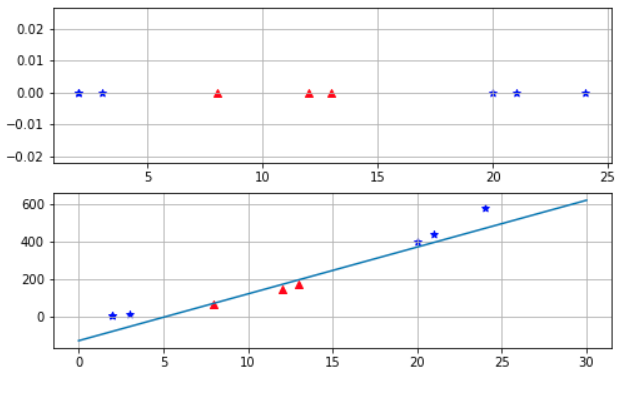
\includegraphics[height=0.3\textheight,width=0.9\textwidth,keepaspectratio]{nonLinearData} \caption{Non-linear data. Here, the function is $\phi : \mathbb{R} \to \mathbb{R}^{2}$, with $\phi(x)=(x, x^2)$. } \label{fig:nonLinearData} \end{figure}
  In this new representation, we \textbf{can} linearly separate the samples. Note - we do need to recenter the projected samples. We will write $\phi(\bm{x}^{(i)})$ again assuming it is centered. Another assumption is that $\left\{ \phi(\bm{x}^{(i)}) \right\}_{i=1}^{n}$ are linearly independent. 

Now we can use PCA, only we do so on the new covariance matrix:
\[
  S_{\phi} \stackrel{\text{ def }}{=} \frac{1}{n} \sum_{i=1}^{n} \phi(\bm{x}^{(i)}) \phi( \bm{x}^{(i)})^T
\]
Continuing similarly to PCA, we wish to find the (largest) eigenvectors of $S_{\phi}$. 
If we denote $\mathcal{F}$ dimension by $|\mathcal{F}|$, then $S_{\phi} \in \mathbb{R}^{|\mathcal{F}| \times  |\mathcal{F}|}$. 
This suggest a new problem - if $|\mathcal{F}| >> n$, then computations become expensive. Luckily, we notice that:

\begin{theorem}[The kernel theorem] \hphantom{}

  \noindent\fbox{\parbox{\textwidth}{Computing the (nonzero) eigenvectors of $S_{\phi}$ requires only knowing the inner products
\[
  k(\bm{x}^{(i)}, \bm{x}^{(j)} ):=  \big\langle \, \phi(\bm{x}^{(i)}) \,, \, \phi(\bm{x}^{(j)}) \, \big\rangle
\]
  Hence, if computing $k(\bm{x}^{(i)}, \bm{x}^{(j)})$ can be done easily, then we reduced the complexity of the problem}} 

\begin{proof}
We will first prove a lemma.
\begin{lemma}{Range of $S_{\phi}$}:  Recall that:
\[
  S_{\phi} = \frac{1}{n} \sum_{i=1}^{n} \phi(\bm{x}^{(i)}) \phi(\bm{x}^{(i)})^T
\]
Let $\bm{w} \in \mathcal{F}$ be any vector. Then:
\[
S_{\phi} \bm{w} = \frac{1}{n} \sum_{i=1}^{n} \phi(\bm{x}^{(i)}) \phi(\bm{x}^{(i)})^T \bm{w} = \frac{1}{n} \sum_{i=1}^{n} \phi(\bm{x}^{(i)}) \, \langle \, \phi(\bm{x}^{(i)}) \,, \bm{w} \, \rangle
\]
Therefore, $S_{\phi} \bm{w}$ is a linear combination of $\{  \phi(\bm{x}^{(i)}) \}_{i=1}^{n}$, with the coefficients being  $\alpha_i= \langle \, \phi(\bm{x}^{(i)}), \bm{w} \, \rangle$. 
From the assumption that $\left\{  \phi(\bm{x}^{(i)}) \right\}_{i=1}^{n}$ are linearly independent, this representation is unique. 
\end{lemma}

Continuing the proof: denote by $\bm{v}$ a (yet unknown) eigenvector of $S_{\phi}$, i.e.:
\begin{equation} \label{eq:kernelEigenvectorDef}
  S_{\phi} \bm{v} = \lambda \bm{v}
\end{equation}
Using the lemma, we can write:
  \begin{equation} 
  \bm{v} = \sum_{j=1}^{n} \alpha_{j} \phi(\bm{x}^{(j)})
\end{equation}

Where $\alpha_j  \in \mathbb{R}, \alpha_j = \langle \, \phi(\bm{x}^{(j)}) \,, \, \bm{v} \, \rangle$ are the coefficients we wish to determine. We write $\bm{\alpha}=[\alpha_{1}, \ldots, \alpha_n]^T$.  Plugging this into~\cref{eq:kernelEigenvectorDef}, we get:
\begin{align*}
  S_{\phi} \bm{v} &= \frac{1}{n} \Big( \sum_{i=1}^{n} \phi(\bm{x}^{(i)}) \phi(\bm{x}^{(i)})^T \Big)  \bm{v} \\
  &= \frac{1}{n} \Big( \sum_{i=1}^{n} \phi(\bm{x}^{(i)}) \phi(\bm{x}^{(i)})^T \Big)  \sum_{j=1}^{n} \alpha_j \phi(\bm{x}^{(j)})  \\
  &= \frac{1}{n} \sum_{i=1}^{n} \phi(\bm{x}^{(i)}) \sum_{j=1}^{n} \alpha_{j} \langle \, \phi(\bm{x}^{(i)}) \,, \, \phi(\bm{x}^{(j)}) \, \rangle
\end{align*}
Define a new matrix $K \in \mathbb{R}^{n \times  n}$ by:
\[
  K_{ij} = \langle \, \phi(\bm{x}^{(i)}), \phi(\bm{x}^{(j)}) \, \rangle
\]

[Note - we've assumed that $\phi$ sends such that $\{  \phi(\bm{x}^{(i)}) \}_{i=1}^{n}$ are centered. Another way to have this, is to define $\overline{K} = K - \frac{1}{n}\bm{1}^{T} K - \frac{1}{n}K\bm{1} + \frac{1}{n^2} \bm{1}^{T} K \bm{1}$, i.e. subtract row and col mean, and add total mean to remedy over correction.] 

Then we get that:
\begin{align*}
  S_{\phi} \bm{v} = \frac{1}{n} \sum_{i=1}^{n} \phi (\bm{x}^{(i)}) \sum_{j=1}^{n} \alpha_{j} \overline{K}_{ij} = \frac{1}{n} \sum_{i=1}^{n} \phi(\bm{x}^{(i)}) (\overline{K} \bm{\alpha})_{i}
\end{align*}

Developing the RHS of~\cref{eq:kernelEigenvectorDef}, we have:
\[
  \lambda \bm{v} = \lambda \sum_{i=1}^{n} \alpha_i \phi(\bm{x}^{(i)})
\]
Rewriting~\cref{eq:kernelEigenvectorDef}, we get:
\[
   \frac{1}{n} \sum_{i=1}^{n} \phi(\bm{x}^{(i)}) (\overline{K} \bm{\alpha})_{i}
= \lambda \sum_{i=1}^{n} \alpha_i \phi(\bm{x}^{(i)})
\]
From the linear independence of $\left\{ \phi(\bm{x}^{(i)}) \right\}_{i=1}^{n}$, we know the coefficient for each $\phi(\bm{x}^{(i)})$ must be equal, hence we get:
\begin{align*}
  &  \frac{1}{n} (\overline{K} \bm{\alpha})_i = \lambda \alpha_i \\
  \Rightarrow \ & \big( \overline{K} \bm{\alpha} \big)_i = n \lambda \alpha_i \\
  \Rightarrow \ & K \bm{\alpha} = n \lambda \bm{\alpha}
\end{align*}
  Therefore, the original problem of finding eigenpairs $(\bm{v}, \lambda)$ for the $|\mathcal{F}| \times |\mathcal{F}|$ matrix $S_{\phi}$, is actually equivalent to finding the eigenpairs $(\bm{\alpha}, n \lambda)$ of the $n \times n$ matrix  $\overline{K}$. Since $|\mathcal{F}| >> n$, the second task is computationally easier. Using kernel function $k$, we compute (centered) matrix $\overline{K}$, find its eigenvalues $\bm{\alpha}_1, \ldots \bm{\alpha}_{n}$ with eigenvalues $n \lambda_1, \ldots, n \lambda_{n}$, and proceed. 
\end{proof}
\end{theorem}

\subsection{Kernel PCA}
We finish by performing kernel PCA, projecting the lifted samples $\phi(\bm{x}^{(i)})$ onto the $m$-th largest eigenvector of the (centered) kernel matrix $\overline{K}$, using \textbf{only the kernel function}:
\[
  k(\bm{x}^{(i)}, \bm{x}^{(j)}) := \langle \phi(\bm{x}^{(i)}, \phi(\bm{x}^{(j)}) \rangle
\]
Let $\bm{\alpha}_{m} = [(\bm{\alpha}_{m})_1, \ldots, (\bm{\alpha}_{m})_n]$ denote the m-th largest eigenvector of the centered kernel matrix $\overline{K}$. 
Denote by $\bm{y}^{(i)} \in \mathbb{R}^{d}$ the embedding of $\bm{x}^{(i)}$ by kernel PCA using the first $d$ largest eigenvectors of $\overline{K}$. 
Let $\bm{v}_{m}$ the m-th largest eigenvector of $S_{\phi}$. 
Remember that $\bm{v}_{m} = \sum_{j=1}^{n} \phi(\bm{x}^{(j)}) \, (\bm{\alpha}_m)_j$. 
Then we have that:
\begin{align*}
  (\bm{y}^{(i)})_{m} =  \langle \, \phi(\bm{x}^{(i)}) \,, \, \bm{v}_{m} \, \rangle &= \langle \, \phi(\bm{x}^{(i)}) \,, \, \sum_{j=1}^{n} \phi(\bm{x}^{(j)}) (\bm{\alpha}_m)_j \, \rangle  \\
  &=  \sum_{j=1}^{n} (\bm{\alpha}_m)_j \, \langle \, \phi(\bm{x}^{(i)}) \,, \, \phi(\bm{x}^{(j)}) \, \rangle \\
  &= \sum_{j=1}^{n} (\bm{\alpha}_{m})_j \overline{K}_{ij} \\
  &= (\overline{K} \bm{\alpha}_{m})_{i} 
\end{align*}
And therefore:
\[
  \begin{bmatrix} | & \ldots & | \\ \bm{y}^{(1)} & \ldots & \bm{y}^{(n)} \\ | & \ldots & | \end{bmatrix} = \begin{bmatrix} - & \bm{\alpha}_1 ^{T} & - \\ & \hdots & \\ - & \bm{\alpha}_{d}^{T} & -  \end{bmatrix} K
\]

We create embeddings using \textbf{only} the kernel function $k$. 

\begin{example}
Consider a dataset consisting of points lying on a circle on $\mathbb{R}^{2}$:
\[
  \bm{x}^{(i)} = \begin{bmatrix} \cos(\theta_i) \\ \sin(\theta_i) \end{bmatrix},  \quad  \theta_i = \frac{2 \pi i}{n}, \quad i=1,\ldots, n
\]
clearly this is a 1 dimensional data, however it currently in $\mathbb{R}^{2}$. Since this data is has a non-linear structure, classic PCA would not help in reducing its dimension. We use the RBF function:
\[
  k(\bm{x}^{(i)}, \bm{x}^{(j)}) = e^{- \frac{\lVert \bm{x}^{(i)} - \bm{x}^{(j)} \rVert }{2 \sigma ^2}} 
\]


For simulation, The un-centered kernel matrix \( K \) is computed for \( n = 100 \) and \( \sigma = 0.5 \).

The kernel matrix is centered as:
\[
  K_\text{centered} = K - \frac{1}{n} \bm{1} K - K \frac{1}{n} \bm{1} + \frac{1}{n} \bm{1} K \frac{1}{n} \bm{1},
\]
where \( \bm{1} \) is the all-ones matrix.

The eigenvalues and eigenvectors of \( K_\text{centered} \) are computed. The eigenvalues in descending order are:
\[
  \lambda_1 = 17.8751, \quad \lambda_2 = 17.8751, \quad \lambda_3 = 11.7627, \ldots
\]

The projection onto the first principal component is given by:
\[
  \bm{z} = K_\text{centered} \bm{v}_1,
\]
where \( \bm{v}_1 \) is the eigenvector corresponding to \( \lambda_1 \).

Below is a plot of the projection:
  \begin{figure}[H] \centering 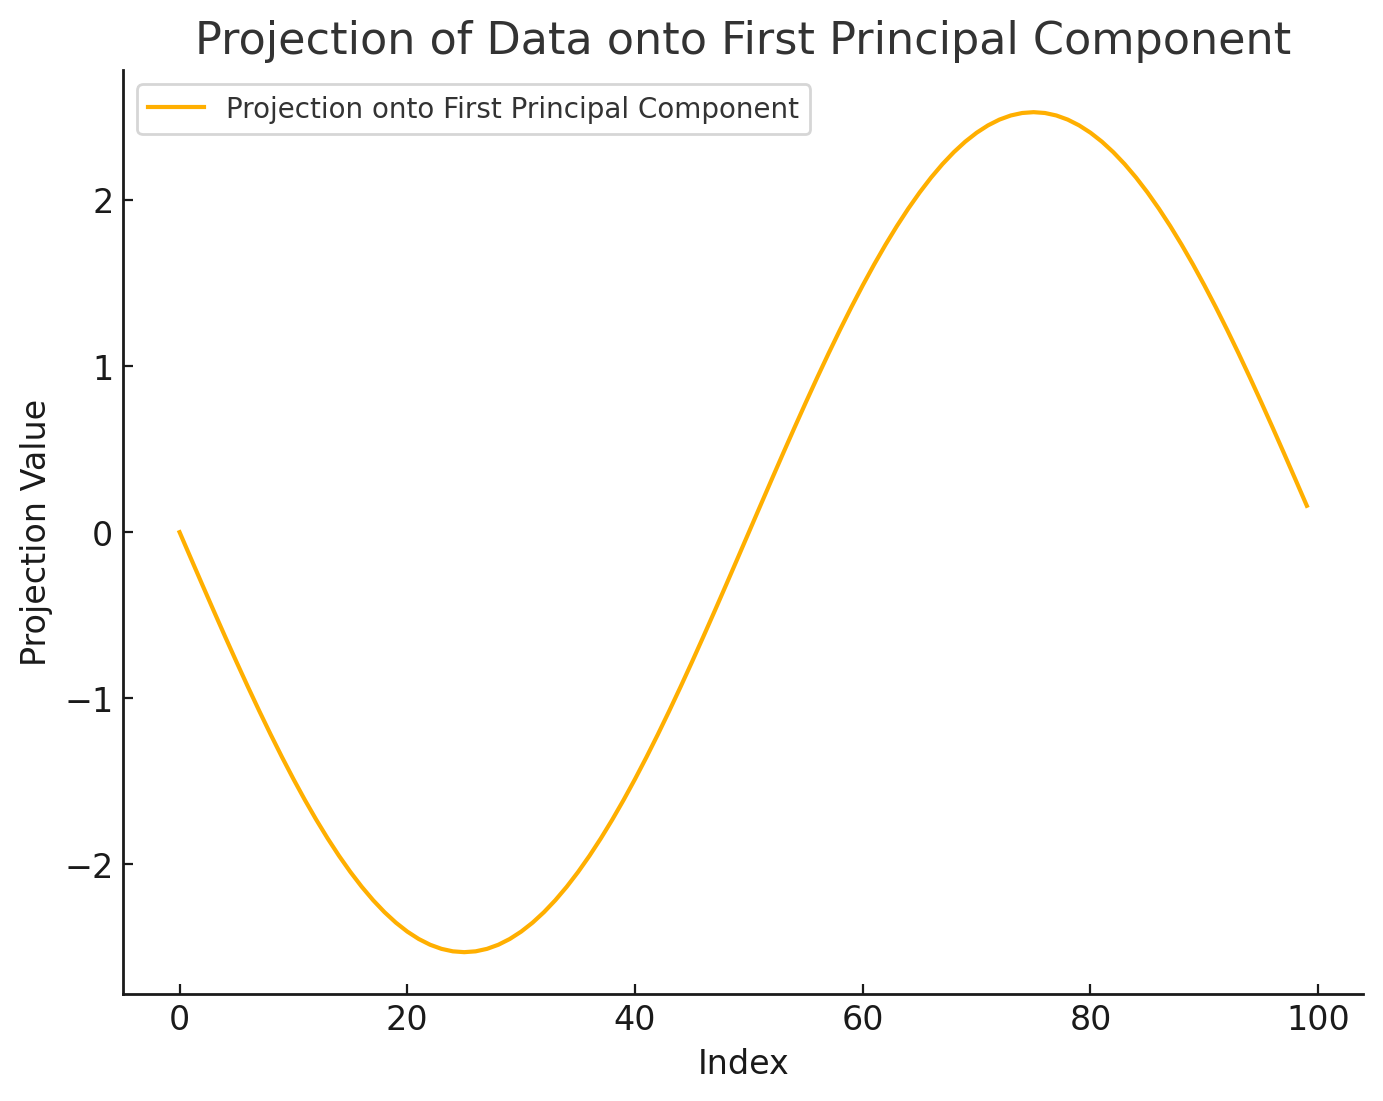
\includegraphics[height=0.2\textheight]{rbfProjection} \caption{Projecting the points on the circle using the largest eigenvector of the centered kernel matrix. Clearly we are projecting $\bm{x}^{(i)}$, associated to $\theta_i$, to a slightly scaled version of $-\sin(\theta_i)$} \label{fig:rbfProjection} \end{figure}
\end{example}



\begin{remark}[(Classic) PCA is linear] (Classic) PCA can only find linear relations in the data. Assume $\bm{x}^{(i)}$ is a sample, and $W \in \mathbb{R}^{k \times d}$ is the projection matrix containing the  $k$ largest eigenvectors of the sample covariance matrix $S = \frac{1}{n} X^T X$. Let $\bm{y}^{(i)}$ denote the projection of $\bm{x}^{(i)}$, i.e.:
\[
  \bm{y}^{(i)} = W \bm{x}^{(i)} 
  \]
Notice we are only applying a linear transformation on $\bm{x}^{(i)}$, hence PCA is linear.

Kernel PCA is nonlinear. 
\end{remark}



\section{Week 2}
\subsection{Encoder Decoder}
Let $x \in \mathbb{R}^{D}$ be some sample. A common task is to do dimensionality reduction,  to some representation $y \in \mathbb{R}^{d}$, and then do reconstruction to $\widetilde{x} \in \mathbb{R}^{D}$. This is an encoder-decoder framework. 
\begin{figure}[H] \centering 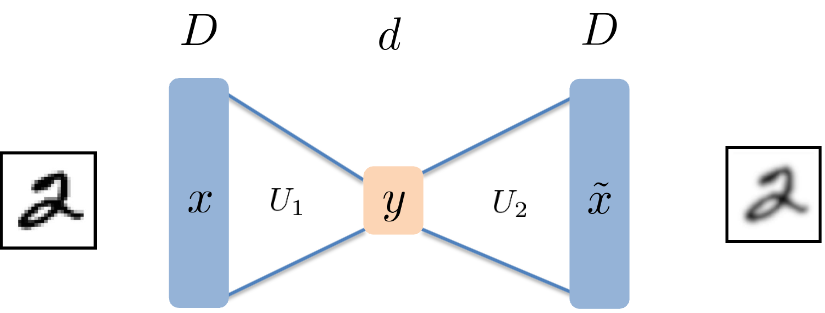
\includegraphics[height=0.3\textheight,width=0.9\textwidth,keepaspectratio]{encoderDecoder}  \label{fig:encoderDecoder} \end{figure}

\begin{itemize}

  \item Setup: Let $X \in \mathbb{R}^{D \times  n}$, where $D$ is number of features and $n$ is number of samples. Assume the data is centered, there are no redundant features, and $n \geq D$, i.e. $\myrank(X) = D$.  Denote by $Y \in \mathbb{R}^{d \times  n}$ an encoding of $X$, and denote by   $\widetilde{X} \in \mathbb{R}^{D \times  n}$ a reconstruction of $X$ using $Y$.
  \item Objective: We wish, using \ul{linear} operators, to find $\widetilde{X}$ s.t. :
  \[
    \min_{\widetilde{X}} \lVert X - \widetilde{X} \rVert_{F}^2
  \]
Since both the encoding and decoding is done via linear operators, we can write:
\[
  \min_{\widetilde{X}} \lVert X - \widetilde{X} \rVert_{F}^2 \ \text{ s.t. } \ \widetilde{X} = U_{2}Y = U_{2} U_{1}X \quad  U_1 \in \mathbb{R}^{d \times  D}, U_2 \in \mathbb{R}^{D \times d}
\]
  \item Solution: PCA. Let $\hat{P} = \frac{1}{n} X X^{T}$ be the covariance matrix, and let $U$ be the first $d$ largest eigenvectors of $\hat{P}$. Then $U_1 = U ^{T}, U_2 = U$. 
  \item \ul{Geometric PCA is not-unique}: Notice that for every orthogonal matrix $R \in \mathbb{R}^{d \times d}$, we have that $U_1 = (UR)^{T}, U_2 = (UR)$ is also a minimizer.  Denote $\widetilde{U}=UR$. 
For example, if our data really only has entries in the first two entries, then we can encode it to $X-Y$ plane. 
However every rotation following this projection would also serve, provided the decoder also includes the inverse rotation. 

I.e. the encoding $Y$ isn't unique.  
However, statistical PCA is unique - how can this be? 
The answer is that in statistical PCA, we add a requirement that there is no correlation between the features (i.e. they are orthogonal), i.e. every row (feature) of $Y$ is uncorrelated with every other row. 
  If $Y = U^{T} X \in \mathbb{R}^{d \times  n}$, then we have that $E[Y Y ^{T}] = \Lambda = \text{diag}(\lambda_1, \ldots, \lambda_{d})$, i.e. the encodings are not correlated. However, for $\widetilde{Y} = \widetilde{U}^{T} X = (UR)^{T} X$, we have that:
\[
  E[\widetilde{Y} \widetilde{Y}^{T} ] = R^{T} \Lambda R
\]
  i.e. there can be non-zero off-diagonal elements, and hence the features can be  correlated, unlike (statistical) PCA. 
\end{itemize}

\subsection{Relating Statistical and Geometrical PCA}


\subsection{SVD, PCA}
\begin{theorem}[SVD] Let $X \in \mathbb{R}^{m \times  n}$, with $m$ samples and $n$ features per sample,  $q = \min \left\{ m,n \right\}$ and $r = \mathrm{rank}(M)$. SVD decomposes $X$ to
\[
  X = U \Sigma V^{T}
\]
with $U \in \mathbb{R}^{m \times m}, \Sigma \in \mathbb{R}^{m \times n}, V \in \mathbb{R}^{n \times n}$.  $\Sigma$ is a rectangular diagonal matrix, with non-increasing entries.  

\end{theorem}


\begin{theorem}[PCA and SVD] Recall that in PCA (assuming $X$ is centered), we compute:
\[
\hat{P} = \frac{1}{n-1} X^{T} X = \frac{1}{n-1} V \Sigma^{T} U ^{T} U \Sigma V^{T} = V \frac{\Sigma ^2}{n-1} V^{T}
\]
  I.e. the right singular vectors in $V$ (from the SVD) are the principal directions (eigenvectors) from PCA, and the PCA eigenvalues $\lambda_i$ are related to $\sigma_i$ via $\lambda_i = \frac{\sigma_i ^2}{n-1}$. 

Since the columns of $V$ are the principal directions, we can project onto them to get principal scores, i.e. an optimal lower dimension embedding. The rank $k$ embedding $Y \in \mathbb{R}^{m \times k}$ is given by:
\[
Y = X V_{n \times  k} = U \Sigma V^{T} V_{n \times k} = U \Sigma_{m \times k} = U_{m \times k} \Sigma_{k \times k}
\]
where:
\[
 \Sigma_{k \times k}  = \text{diag}(\sigma_1, \ldots, \sigma_k) =  \begin{bmatrix} \sigma_1 & 0 & \ldots  & 0 \\ 0 & \sigma_2 & 0 & 0 \\ 0 & \ddots & \ddots & 0 \\ 0 & \cdots & \cdots & \sigma_k  \end{bmatrix}
\]
  Note that $Y = U_{m \times k} \Sigma_{k \times  k}$ are the principal scores. Therefore we can produce a reconstruction $\widetilde{X} \in \mathbb{R}^{m \times n}$ by using the principal scores to take a weighted sum of the principal directions:
\[
  \widetilde{X} = Y (V^{T})_{k \times n} =  (U_{m \times k}   \Sigma_{k \times k}) (V^{T})_{k \times n}
\]
This can be written as:
\begin{align} \label{eq:SVDDecomp}
  \widetilde{X} &= Y (V^{T})_{k \times n} = U_{m \times k} \Sigma_{k \times k} (V^{T})_{k \times n} = \\
  &= U_{m \times k} \begin{bmatrix} - & \sigma_1 v_1^{T} & - \\ - & \vdots & - \\ - & \sigma_k v_k^{T} & - \end{bmatrix} = \sum_{i=1}^{k} \sigma_i u_i v_i^{T}
\end{align}
 Alternatively, we can think of the reconstruction $\widetilde{X}$ of rank k as taking the first $k$ largest singular values, and zeroing the rest. Let $\Sigma^{(k)} \in \mathbb{R}^{m \times n}$ be defined by:
\[
  \Sigma^{(k)}  = \begin{cases} \sigma_i, & i \leq k \\ 0, & i \geq k \end{cases} 
\]

Then:
\[
  \widetilde{X} = U \Sigma^{(k)} V^{T}
\]
This follows from the RHS of~\cref{eq:SVDDecomp}. 

\end{theorem}

\begin{theorem}[Reconstruction Error]
  \[
    \epsilon(k) = \lVert X - \widetilde{X} \rVert_{F}^2 = \Tr \Big( (X - \widetilde{X})^{T} (X - \widetilde{X}) \Big) = \sum_{i=k+1}^{n} \sigma_i ^2
  \]
\end{theorem}

\begin{remark}[Model Selection - How to choose embedding dimension $k$] knee point 
\end{remark}

\subsection{Stochastic Neighbor Embedding}
\begin{definition}[(Shannon) Entropy]  Let $X$ be a discrete random variable which takes values in the set $\mathcal{X}$, with PMF $p: \mathcal{X} \to [0,1]$ such that $p(x) := \mathbb{P}[X = x]$. Then:
  \[
    H(X) = - \sum_{x \in \mathcal{X}} p(x) \log p(x)
  \]
  
\end{definition}

\begin{definition}[KL Divergence] Let $p,q$ be PMF over $\mathcal{X}$. Then:
\begin{align*}
  D(p||q) := \sum_{x in \mathcal{X} } p(x) \log \frac{p(x)}{q(x)}
\end{align*}
\end{definition}

\begin{definition}[Jensen-Shannon Divergence] Symmetric version of the KL-Divergence:
\[
  D_{JS}(p ; q) := \frac{1}{2} \big( D(p || \rho) + D(q ||  \rho)  \big)
\]
where:
\[
  \rho = \frac{1}{2} (p+q)
\]
\end{definition}

Let $X = \left\{  x_1, \ldots, x_n \right\} \in \mathbb{R}^{D}$
and a distance measure $\lVert x_i - x_k \rVert$. 

\begin{definition}["Conditional Probability"] 
Define "conditional probability":
\[
  p_{j | i } := \frac{\exp{(- \lVert  x_i -x_j \rVert ^2 / 2 \sigma ^2 }) }{\sum_{k \neq  i } \exp (- \lVert x_i-x_k \rVert ^2 / 2 \sigma ^2 )}
\]
This is the Heat-Kernel Affinity. We define $p_{i|i} := 0$ (convention). 
  Let $E$ be the symmetric matrix defined by $E_{ij}=e^{- \lVert x_i -x_j \rVert ^2}.$ Define the non-symmetric matrix $P_{ji} = p_{j|i}$ which is $E_{ji}$ divided by entire $
  i$-th column of$E$. Therefore the columns sum to$1$, but the rows don't. 

\begin{itemize}
\item \ul{Probability Measure} This is a probability measure, since $\sum_{j} p_{j|i} = 1$
  \item \ul{Non-Symmetric} $p_{j|i} \neq p_{i|j}$. Example: Imagine three points $a < b < c$ on a line, with b in the middle. Then $p_{b|a} > p_{a | b}$, since $b$ has other close neighbors (more popular) than $a$.  
  \item  \ul{Distance} $p_{i|j}$ transforms the euclidean distance $\lVert x_i - x_j \rVert$ into a probability measure. Low distance = High probability (of being neighbors). This allows us to turn the problem of finding similar embeddings into finding similar probability distributions $P$ and $Q$.
\end{itemize}
\end{definition}
 


\begin{theorem}[SNE Embedding] We wish to find low dimensional representation $Y = \left\{ y_1, \ldots  y_n \right\} \in \mathbb{R}^{d}$ with $d << D$, where we measure affinity $q_{j|i}$ by:
\[
  q_{j | i } := \frac{\exp{(- \lVert  y_i -y_j \rVert ^2 }) }{\sum_{k \neq  i } \exp (- \lVert y_i-y_k \rVert ^2  )}
\]
(some omit the $\sigma$ in $q$),  and:
\begin{gather*}
  P_{i} := p_{\cdot | i} = (p_{1|i}, \ldots, p_{n|i}) \\
  Q_{i} := q_{\cdot | i} = (q_{1|i}, \ldots, q_{n|i})
\end{gather*}
Thus $P_{i}$ is the normalized similarity vector for $x_i$, and defines a conditional probability distribution. 

We wish that $y_i$ is similar to $x_i$. 
\end{theorem}

\begin{definition}[Perplexity] $\sigma_i$ is chosen using perplexity, with:
\[
  \text{Perp}(P_{i}) : = 2^{H(P_i)} \quad \text{with } H(P_i) := - \sum_{j \neq i} p_{j|i} \log_{2} p_{j|i}
\]
  $\text{Perp}(P_i)$ is a smooth measure of the effective number of neighbors of $x_i$. 
\end{definition}


\begin{definition}[SNE Cost Function] 
  Define the Cost Function, that minimizing it  aims to maintain neighborhood similarity:
\[
 C(Y) = C( \left\{ y_i \right\}) = \sum_{i} KL(P_i | Q_i) = \sum_{i} \sum_{j \neq i} p_{j | i} \log \frac{p_{j|i}}{q_{j|i}}
\] 
We look for:
\[
  \min_{Y} C(Y)  
\]
\begin{itemize}

  \item \ul{Goal}: Goal of SNE is to minimize mismatches between $p_{j|i}$ and $q_{j|i}$. 
 SNE minimizes the sum of KL divergences over all data points, using a gradient descent method. We denote the cost function $C$:
  \item \ul{Non-Symmetry}: For \textbf{close} points ($p_{j|i}$ high) there is \textbf{high} cost for mapping them \textbf{far} (i.e. small $q_{j|i}$). However, for \textbf{far} points ($p_{j|i}$ low), there is \textbf{small} cost for mapping them close (i.e. assigning high $q_{j|i}$). This leads to asymmetry, where SNE preserves \textbf{local} structure, but not \textbf{global} structure. 
\end{itemize}
\end{definition}

\begin{theorem}[Cost Function Gradient] in Tirgul. 
\[
  \frac{\partial C}{\partial y_i} = 2 \sum_{j} \big( p_{j|i} - q_{j|i} + p_{i|j} -q_{i|j} \big)( y_i - y_j)
\]
\end{theorem}


\begin{theorem}[SNE Gradient Descent] \hphantom{}
\begin{itemize}

  \item We initialize  $y$ by sampling map points randomly from an isotropic Gaussian with small variance that is centered around the origin. 
  \item A relatively large momentum is added to gradient to avoid poor local minima. Alternatively, the current gradient is added to an exponentially decaying sum of previous gradients.
  \[
    \mathcal{Y}^{(t)} = \mathcal{Y}^{(t-1)} + \eta \frac{\partial C}{\partial y} + \alpha(t) (\mathcal{Y}^{(t-1)} + \mathcal{Y}^{(t-2)} ) 
  \]
  where $\alpha(t)$ is the momentum at iteration $t$ and $\eta$ is the learning rate.  

\end{itemize}

\end{theorem}


\begin{remark}[SNE Notes] \hphantom{}
\begin{itemize}

  \item t-SNE is good for visualization, not necessarily as input to a downstream . It does not preserve global structure. 
  \item t-SNE is nonlinear.
  \item t-SNE \ul{does not} preserve distances. Close points will behave similarly, however, more global structure is not preserved. E.g. let $x$ be our base points, and $x_1, x_2$ two points with $d(x_1-x) < d(x_2-x)$. Then it's not necessarily true that $d(y_1-y) < d(y_2-y)$, where $y,y_1,y_2$ are the t-SNE embeddings. If that's a goal, then use MDS. Intuitively, PCA \href{https://stats.stackexchange.com/a/176801/213861}{preserves large pairwise distances, but not small pairwise distances}. t-SNE does not aim to preserve any (global) distances. 
  \item T-SNE is designed to preserve local similarities between data points, which means it excels at revealing clusters and local patterns in high-dimensional data. However, this focus on local structure comes at the expense of accurately representing global relationships.
 \item  Probability Distribution: T-SNE uses a heavy-tailed Student t-distribution in the low-dimensional space, which tends to push apart points that are not similar

\end{itemize}
\end{remark}

\subsection{t-SNE}
\ul{Crowding Problem} Mapping far $x_i$ points to nearby (crowded) $y_i$  points in the embedding dim is both problematic, and makes gradient descent unstable. Specifically, think of $x_i, x_j$ being two outliers who are near each other. Then $p_{j|i}$ (and $p_{i|j}$) will be very small, and hence the cost function won't take them into consideration. 

tSNE solves this by using:
\begin{enumerate}

  \item \ul{Symmetry}: uses a symmetrized version of the SNE cost function, with simpler gradients.
  \item \ul{Student-t distribution}: Uses Student-t distribution instead of a Gaussian to compute the \textit{similarity} in the low-dimensional space. A heavy-tailed distribution goes to zero slower than an exponential. This will give outliers high values.  

\end{enumerate}


\ul{Solving Asymmetry} We can do \textbf{symmetric SNE}, by taking the denominator with respect to all pairwise possibilities. We write:
\[
  p_{ij} := \frac{\exp(- \lVert x_i -x_j \rVert^2 / 2 \sigma ^2) } {\sum_{k} \sum_{\ell \neq k } \exp(- \lVert x_k - x_{\ell} \rVert ^2 / 2 \sigma ^2 ) }
\]

Recall that previously, $P_{ji}=p_{j|i}$ was given as $E_{ji}$ divided by the $i$-th row of $E$. Now instead, $P_{ji}$ is defined to be $E_{ji}$ divided by the \textit{entire} matrix $E$ (which has a zero main diagonal), and therefore $P_{ji}=P_{ij}$. 
In the \textit{low-dimensional} map $q_{i|j}$ as  the denominator ($Z_i$) by pairwise similarities:
\[
  q_{ij} := \frac{e^{- \lVert y_i -y_j \rVert^2 } } {\sum_{k} \sum_{\ell \neq k } e^{- \lVert y_k - y_{\ell} \rVert ^2}   } 
\]

However, this still does not solve the crowding problem. $p_{ij}$ can still be arbitrarily small, which is problematic. Therefore, tSNE uses a different conditional probability:
  \[
    p_{ij} := \frac{p_{i|j} + p_{j|i}}{2n}
  \]
This \ul{symmetric} definition ensures that:
\[
  \sum_{j} p_{ij} > \frac{1}{2n}
\]
i.e. $p_{ij}$ is bounded below, regardless of how much of an outliers $x_i$ and $x_j$ are, and therefore $y_i$ and $y_j$ will have to be somewhat reasonable.  


\ul{Heavy-Tail} Additionally, to solve the crowding problem, we give more weight to outliers, by using for the mapping $q_{ij}$ a heavy-tailed distribution instead of the Gaussian. Specifically we use the Student-t distribution:
\[
  q_{ij} := \frac{(1 + \lVert y_i-y_j \rVert ^2)^{-1} }{ \sum_{k} \sum_{\ell \neq  k } (1 + \lVert y_k - y_j \rVert ^2 ) ^{-1}}
\]

The heavy tails "allows" the map to place points further apart. 



\subsection{Canonical Correlation Analysis (CCA)}
The idea is to reduce the number of variables without sacrificing too much information. 
Whereas PCA deals with random variables that come from a single set, CCA assumes the variables come from \textbf{two} sets. We select an uncorrelated linear combination of the two sets of variables, which are pairwise highly correlated.

We assume wlog that $E[X] = E[Y] = 0$. Additionally, We assume both random vectors have no redundant features, i.e. no features that can be expressed as a linear combination of the others. This gives that $XX^{T}$ and $YY^{T}$ are (strictly) positive definite (and not \textit{semi}-positive definite). 

\ul{Objective}: Given multivariate random vectors $X \in \mathbb{R}^{n}, Y \in \mathbb{R}^{m}$, find \textit{linear} mappings, $a \in \mathbb{R}^{n}, b \in \mathbb{R}^{m}$, also known as the (first) \textbf{canonical directions}, such that for the random variables $U = a^{T}X$ and $V = b^{T}Y$, we have:
\begin{equation} \label{CCAObjective1}
\begin{aligned}
  & \max_{a,b} \big[ (a^{T} X) (b^{T} Y) \big] \\
  & \operatorname*{\text{subject to}} \quad  E \left[ (a^{T}X)^2 \right] = 1 \,, \  E \left[ (b^{T}Y)^2 \right] = 1 
 \end{aligned}
\end{equation}

Denoting $\Sigma_{XX} :=E[X X^{T}]$ and $\Sigma_{YY} := E[Y Y^{T}]$ and $\Sigma_{XY} := E[X Y^{T}], \Sigma_{YX} := E[Y X^{T}]$ 
our objective becomes
\begin{align} \label{eq:CCAObjective2}
& \max_{a,b} a^{T} \Sigma_{XY} b \\ 
  & \text{ s.t. } a^{T} \Sigma_{XX}a = 1 \, \ b^{T} \Sigma_{YY} b = 1 \label{eq:CCAConstraints}
\end{align}

Note that:
\[
  E[a^{T} X] = a^{T} E[X] = 0
\]
and similarly $E[b^{T} Y] = 0$. 

Define:
\[
  M \stackrel{\text{ def }}{=}  \Sigma_{XX}^{-1/2} \Sigma_{XY} \Sigma_{YY}^{-1/2} \in \mathbb{R}^{n \times  m}  
\]
Then we have:
\[
  MM' = \Sigma_{XX}^{-1/2} \Sigma_{XY} \Sigma_{YY} ^{-1} \Sigma_{XY}^{T} \Sigma_{XX}^{-1/2} \ \in \mathbb{R}^{n \times n} \quad, \quad  M'M   = \Sigma_{YY}^{-1/2} \Sigma_{XY}^{T} \Sigma_{XX} ^{-1} \Sigma_{XY} \Sigma_{Y}^{-1/2}
\]
We've shown that $MM', M'M$ are PD and have the same eigenvalues. 

Define:
\[
  B = \Sigma_{XX} ^{-1} \Sigma_{XY} \Sigma_{Y}^{-1} \Sigma_{XY}^{T} \quad, \quad  C = \Sigma_{YY} ^{-1}  \Sigma_{XY}^{T} \Sigma_{XX} \Sigma_{XY}
\]

We note that
\begin{gather}
  B = \Sigma_{XX}^{-1/2} MM^{T} \Sigma_{XX}^{1/2} \label{eq:CCABasMMT} \\
  C = \Sigma_{YY}^{-1/2} M^{T} M \Sigma_{YY}^{1/2} \label{eq:CCACasMTM}
\end{gather}
i.e. $B$ is \textit{similar} to $MM^{T}$ and hence they have the same eigenvalues. Likewise, $C$ is similar to $M^{T}M$, and hence $MM^{T}, M^{T}M,B,C$ all have the same eigenvalues $\lambda_1 > \ldots > \lambda_{r} > 0$, where $r$ is the rank of $\Sigma_{XY}$.  


We Solve~\cref{eq:CCAObjective2} using Lagrange Multipliers. Define:
\[
  L(\rho_{x}, \rho_{y}, a,b) := a^{T} \Sigma_{XY} b - \frac{\rho_{x}}{2} ( a^{T} \Sigma_{XX} a)  - \frac{\rho_{y}}{2} (b^{T} \Sigma_{YY} b)
\]
Differentiating $L$ and looking for stationary points, we get:
\begin{gather}
  \bm{\nabla}_{a} L = \Sigma_{XY} b - \rho_{x} \Sigma_{XX} a = \bm{0} \label{eq:CCADer1} \\
  \bm{\nabla}_{b} L = \Sigma_{XY}^{T} a - \rho_{y} \Sigma_{YY} b = \bm{0} \label{eq:CCADer2}
\end{gather}
We pre-multiply by $a^{T}$ and $b^{T}$ respectively, and we get:
\begin{gather}
  a^{T}\Sigma_{XY} b = \rho_{x} a^{T} \Sigma_{XX} a = \rho_{x} \label{eq:CCADer3}  \\
  b^{T} \Sigma_{XY}^{T} a = b^{T} \rho_{y} \Sigma_{YY} b  = \rho_{y} \label{eq:CCADer4}
\end{gather}
where we've used~\cref{eq:CCAConstraints}. Therefore we get that $\rho_{x}=\rho_{y}=\rho$. 

Since we've assumed $\Sigma_{XX}, \Sigma_{YY}$ are (strictly) positive definite, they are invertible, and therefore from~\cref{eq:CCADer1} and~\cref{eq:CCADer2}, we get:
\begin{equation}
  a = \frac{\Sigma_{XX} ^{-1} \Sigma_{XY} b}{\rho} 
\end{equation}
Plugging this into~\cref{eq:CCADer2}, we get:
\begin{align*}
  &\frac{1}{\rho} \Sigma_{XY}^{T} \Sigma_{XX} ^{-1}  \Sigma_{XY} b = \rho \Sigma_{YY} b  \\
  \Rightarrow \  & \Sigma_{YY} ^{-1} \Sigma_{XY}^{T} \Sigma_{XX} ^{-1}  \Sigma_{XY} b = \rho ^2 b  \\
  \Rightarrow \ & Cb = \rho ^2 b \label{eq:CCAOptSolC}
\end{align*}

In an analogous way we get:
\begin{equation*} 
  Ba = \rho ^2 a  
\end{equation*}
Therefore we get that the optimal $\hat{a}, \hat{b}$ would be the largest eigenvector of $B$ and $C$, respectively. The reasoning is like in PCA. 

Further, note that:
\begin{align} \label{eq:CCAOptSolB}
  & B \hat{a}  = \rho ^2 \hat{a}   \\
   \Rightarrow \ & MM^{T} (\Sigma_{XX}^{1/2} \hat{a} ) = \rho ^2 (\Sigma_{XX}^{1/2} \hat{a}  ) 
\end{align}
Denote $\hat{u} = \Sigma_{XX}^{1/2} \hat{a}$. Then $\hat{u}$ is an eigenvector of $B$ with eigenvalue $\rho ^2$. Since we've shown that $MM^{T}$ and $B$ have the same eigenvalues, we get that $\hat{u}$ is the largest eigenvector of $MM^{T}$. Therefore, In order to compute $\hat{a}$, all we need to do is find largest eigenvector $MM^{T}$, i.e. $\hat{u}$, and then compute $\hat{a} = \Sigma_{XX}^{-1/2} \hat{u}$. 
Similarly, if $\hat{v}$ is largest eigenvector of $M^{T}M$, then $\hat{b} = \Sigma_{YY}^{-1/2} \hat{v}$. 

Therefore, we can obtain the canonical directions using the eigenvalues of $MM^{T}, M^{T}M$. 


\end{document}
